\documentclass{article}
\usepackage[utf8]{inputenc}
\usepackage{tikz}
\usepackage{geometry}
\geometry{a4paper, margin=1in}
\usetikzlibrary{shapes.geometric, arrows.meta, positioning, fit, backgrounds, calc}

\begin{document}

\begin{figure}[htbp]
\centering
\resizebox{0.9\textwidth}{!}{%
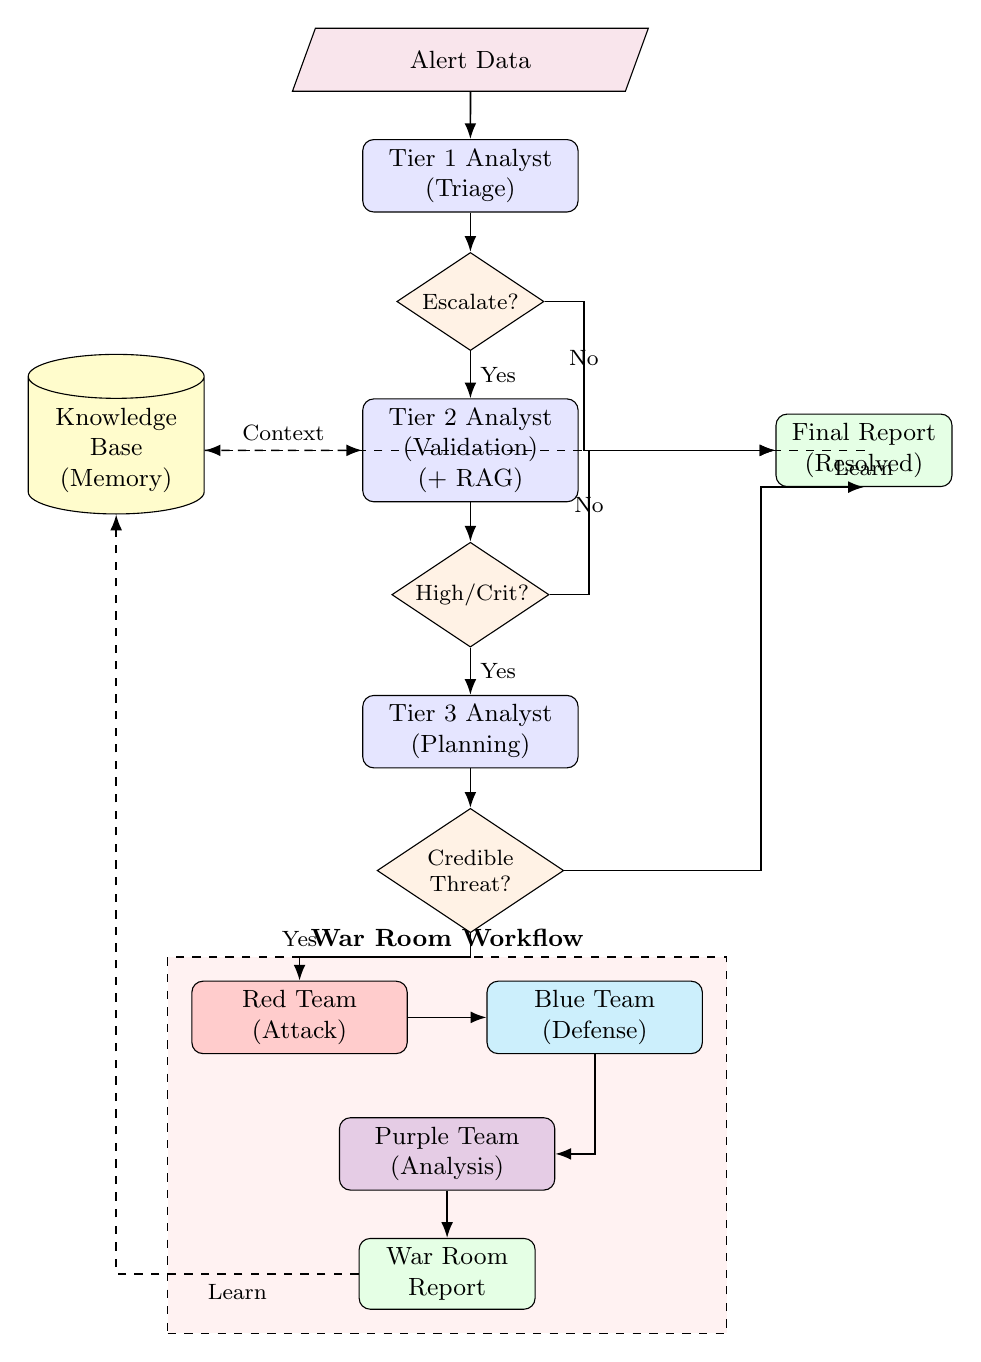
\begin{tikzpicture}[
    node distance = 0.8cm and 1.2cm, 
    proc/.style = {rectangle, draw, fill=blue!10, text width=2.5cm, align=center, minimum height=0.8cm, rounded corners, font=\small},
    decision/.style = {diamond, draw, fill=orange!10, text width=1.4cm, align=center, aspect=1.5, font=\footnotesize, inner sep=1pt},
    term/.style = {rectangle, draw, fill=green!10, text width=2.0cm, align=center, minimum height=0.8cm, rounded corners, font=\small},
    io/.style = {trapezium, trapezium left angle=70, trapezium right angle=110, draw, fill=purple!10, text width=2.0cm, align=center, minimum height=0.8cm, font=\small},
    db/.style = {cylinder, shape border rotate=90, draw, fill=yellow!20, aspect=0.25, text width=2.0cm, align=center, minimum height=1.5cm, font=\small},
    line/.style = {draw, -{Latex[length=2mm]}, semithick},
    subproc/.style = {rectangle, draw, dashed, fill=red!5, inner sep=0.3cm}
]

    % Nodes - Main Column
    \node (start) [io] {Alert Data};
    \node (tier1) [proc, below=0.6cm of start] {Tier 1 Analyst\\(Triage)};
    \node (dec1) [decision, below=0.5cm of tier1] {Escalate?};
    
    \node (tier2) [proc, below=0.6cm of dec1] {Tier 2 Analyst\\(Validation)\\(+ RAG)};
    \node (dec2) [decision, below=0.5cm of tier2] {High/Crit?};
    
    \node (tier3) [proc, below=0.6cm of dec2] {Tier 3 Analyst\\(Planning)};
    \node (dec3) [decision, below=0.5cm of tier3] {Credible\\Threat?};
    
    % Memory / Knowledge Base Node
    \node (kb) [db, left=2.0cm of tier2] {Knowledge Base\\(Memory)};

    % Final Report
    \node (end) [term, right=2.5cm of tier2] {Final Report\\(Resolved)};
    
    % War Room Subgraph
    \node (red) [proc, below left=1.0cm and 0.2cm of dec3, fill=red!20] {Red Team\\(Attack)};
    \node (blue) [proc, right=1.0cm of red, fill=cyan!20] {Blue Team\\(Defense)};
    \node (purple) [proc, below=0.8cm of $(red.south)!0.5!(blue.south)$, fill=violet!20] {Purple Team\\(Analysis)};
    \node (war_room_end) [term, below=0.6cm of purple] {War Room\\Report};

    % Container for War Room
    \begin{scope}[on background layer]
        \node [subproc, fit=(red) (blue) (purple) (war_room_end), label={[font=\bfseries\small]north:War Room Workflow}] (wr_box) {};
    \end{scope}

    % Edges - Main Flow
    \path [line] (start) -- (tier1);
    \path [line] (tier1) -- (dec1);
    
    % Decision 1
    \path [line] (dec1) -- node [right, font=\footnotesize] {Yes} (tier2);
    \path [line] (dec1.east) -- ++(0.5,0) |- node [near start, above, font=\footnotesize] {No} (end.west);
    
    % Memory Interactions
    \path [line, dashed] (kb) -- node [above, font=\footnotesize] {Context} (tier2);
    \path [line, dashed] (end) |- node [near start, below, font=\footnotesize] {Learn} (kb);
    \path [line, dashed] (war_room_end) -| node [near start, below, font=\footnotesize] {Learn} (kb);

    % Decision 2
    \path [line] (tier2) -- (dec2);
    \path [line] (dec2) -- node [right, font=\footnotesize] {Yes} (tier3);
    \path [line] (dec2.east) -- ++(0.5,0) |- node [near start, above, font=\footnotesize] {No} (end.west);
    
    % Decision 3
    \path [line] (tier3) -- (dec3);
    \draw [line] (dec3.south) -- ++(0,-0.3) -| (red.north) node [midway, above, font=\footnotesize] {Yes};
    \draw [line] (dec3.east) -- ++(2.5,0) |- (end.south);
    
    % War Room Internal
    \path [line] (red) -- (blue);
    \path [line] (blue) |- (purple);
    \path [line] (purple) -- (war_room_end);

\end{tikzpicture}
}
\caption{Agentic SOC Workflow with Memory Integration}
\label{fig:soc_workflow_memory}
\end{figure}

\end{document}
